
\documentclass[a4paper]{article}
\usepackage{pslatex}
\usepackage[T1]{fontenc}
\usepackage[utf8x]{inputenc}
\setlength\parskip{\medskipamount}
\setlength\parindent{0pt}
\usepackage{graphicx}
\usepackage{amssymb}
\usepackage{lscape}
%\usepackage{hyperref}

\usepackage{multicol}

\makeatletter

\providecommand{\boldsymbol}[1]{\mbox{\boldmath $#1$}}
\newcommand{\ASL}			{ASL}
\newcommand{\OSC}[1]		{\texttt{#1}}
\newcommand{\lra}			{$\leftrightarrow$}
\newcommand{\seg}[1]		{Seg(#1)}

\setlength{\parskip}{1mm}

\makeatother

\begin{document}

\title{FaustPlayground \\ v.1.0}

\author{Grame, Centre National de Création Musicale\\
{\small <research@grame.fr>} \\
\vspace{2mm}
[ANR-12-CORD- 0009] and [ANR-13-BS02-0008]
}

\maketitle

\topskip0pt

\newpage
\tableofcontents

\newpage
\section{General Considerations}

\subsection{FaustPlayground}
FaustPlayground is a web platform aiming to create patchs of Faust applications and export the patch as a unique application through the FaustWeb compilation service. \\

The FaustPlayground is an extension of the Web Audio Playground by Chris Wilson : http://webaudioplayground.appspot.com/ \\

Two versions of the interface have been created :
\begin{itemize}
\item The pedagogical version aims to introduce the notion of programmation to the young public, through the creation of an audio application. This application can be downloaded on a smartphone, once created.

\item The "normal" version is for every Faust user wanting to try online some  Faust examples, create patchs and use the export interface to FaustWeb service.
\end{itemize}

\subsection{Code Structure}

The scene is the principal element of the FaustPlayground. It is an audio and graphical container. The scene is implemented following the C++ class model, describing a serie of functions that can be executed on it (c.f. SECTION ??).

For the needs of both playgrounds, various scene instances are created:
\begin{itemize} 
\item For the pedagogical version: Accueil, Pedagogie, Finish
\item For the normal version: Playground
\end{itemize}

Those files implement specific functions creating the graphical elements to be added to the specific scene.
For each scene, we have three main functions :
\begin{itemize}
\item init: create the graphical elements
\item onload: callback whenever the scene is loaded in the page
\item onunload: callback whenever the scene is unloaded from the page
\end{itemize}
 
 Main.js handles the different scenes of the application and the navigation between them. \\
 
 The second main element of the FaustPlayground is the notion of Module, representing a Faust application and its interface.
 
 A global view of the interactions between files and data structures is presented in the appendix (c.f. SECTION ). 

\section{SceneClass.js}

\subsection{Class Description}
The SceneClass is an audio and graphical container for Modules. \\

In order to create a scene, you will have to call: {\it createScene(identifier, onload, onunload)}\\
The identifier will become the identifier of the container DIV. Onload/Onunload are callbacks for whenever the scene is loaded/unloaded from the page.

The fields of this class are:
\begin{itemize}
\item Input/Output: intermediate input/output Faust Modules to simplify mute/unmute scene
\item Modules: list of modules contained in the scene
\end{itemize}

The public methods are:
\begin{itemize}
\item Delete scene
\item Add Input/ Add Output: add audio input/output Faust Modules
\item Integrate scene: integrate scene to the page
\item Show/hide
\item Mute/unmute: connect/disconnect scene Input/Output to the WebAudio Context Input/Output
\item Add/Remove module
\item Get Modules
\item Clean Modules
\item Start/stop scene: execute onload/onunload callbacks
\item Get scene container
\item Get Input / get Output
\item Save/Recall scene: Through a Json Description, the scene can be saved and recalled (c.f SECTION ??)
\end{itemize}

\subsection{Scenes Instances}
\subsubsection{Pedagogical Version}
In the pedagogical version, 3 scenes are created: Accueil, Pedagogie and Finish.
They correspond to the graphical menus in which we navigate in the pedagogical FaustPlayground.

\subsubsection{Normal Version}
In the normal version, a unique scene is created: Playground.

\section{Main.js}

 Main.js handles the different scenes of the application and the navigation between them, through the following functions:
 \begin{itemize}
 \item createAllScenes: initialize all the scenes that will be needed by the application
 \item showFirstScene: load default Scene
 \item nextScene/previousScene: navigate in the scenes
\end{itemize}

Main.js also handles the creation of the modules:
 \begin{itemize}
 \item createFaustModule: create Module and add it to current scene
 \item compileFaust: uses libfaust.js to compile the Faust expression. Once the factory is returned, a callback is executed whether it's {\it createFaustModule} in the case of a new module or {\it module.update} in the case of an existing module. \\
 
 The step of compilation is executed first and outside the Module Class. In case it fails, then we don't have to delete an already created module.
\end{itemize}

The reaction to a drop on the page, is handled by:
 \begin{itemize}
 \item setGeneralDragAndDrop
 \item resetGeneralDragAndDrop
 \item uploadFile
 \item uploadOn
 \item terminateUpload
\end{itemize}

And finally the activation of the physical audio input/output:
 \begin{itemize}
 \item activateAudioInput
 \item getDevice
 \item activateAudioOutput
 \end{itemize}

\section{ModuleClass.js}

The Module represents a Faust application and its interface. 
This hand-made class might not be very well dividing the graphical from the structural aspects. 

Its Fields:
\begin{itemize}
\item Graphical elements
\item Graphical In/Output Nodes 
\item Name
\item Code Source
\item DSP
\item Params
\item In/Output Connections: The connections are structures containing a source, a destination and a shape.
\end{itemize}

Private Methods:
\begin{itemize}
\item onDrop 
\item dragCallback
\item dragCnxCallback
\end{itemize}

Public Methods:
\begin{itemize}
\item Delete node
\item Add/remove/get In/output Connections
\item Get In/Output Node
\item Show/hide
\item Get/set Source
\item Get/set Name
\item Get/set/update/delete DSP
\item Edit
\item Update Factory
\item Recompile
\item Create/delete Faust interface: uses the FaustInterface.js file to parse the JSON and create graphical elements
\item Interface callback: called whenever a parameter of the interface is modified by the user
\item Save/recall/get/set/add Params
\item Add/delete/set InputOutput nodes
\item Add/remove listener: listen to a drag event of the module
\item Add/remove connexion listener: listen to drag event starting a connection
\item IsPointIn In/Output
\item IsPointInNode
\end{itemize}



\section{Drag and Connect}
\subsection{Dragging.js}

Dragging.js handles the reaction to the graphical dragging of Modules/Connections with the functions:
\begin{itemize}
\item startDragging
\item whileDragging
\item stopDragging
\end{itemize}

\subsection{Connect.js}

Connect.js handles the Web Audio connections/disconnections between modules. It also handles the creation/deletion of the connectors:
\begin{itemize}
\item connectModules/disconnectModules/disconnectModule
\item saveConnection
\item createConnection/deleteConnection
\item breakSingleInputConnection
\end{itemize}

\section{Pedagogie}
\subsection{Library.js}

This file contains the function creating the graphical library of the pedagogical version. \\

The Faust resources of the library are for now on the Faust server at faust.grame.fr/www/pedagogie.
To easily scan the content of the library, the file : {\it faust.grame.fr/www/pedagogie/index.json} encodes the resources. \\
Library.js decodes this file to create the graphical interface.

\subsection{Tooltips.js}

To guide the user to take charge of the application, some tooltips appear depending of the situation.
The decision to make them appear and all the tooltip choices are described in this file.

\newpage
\section{Scenario - Example - Pedagogical FaustPlayground}

\subsection{Initialize Pedagogical Playground}
\begin{figure}[!h]
\begin{center}
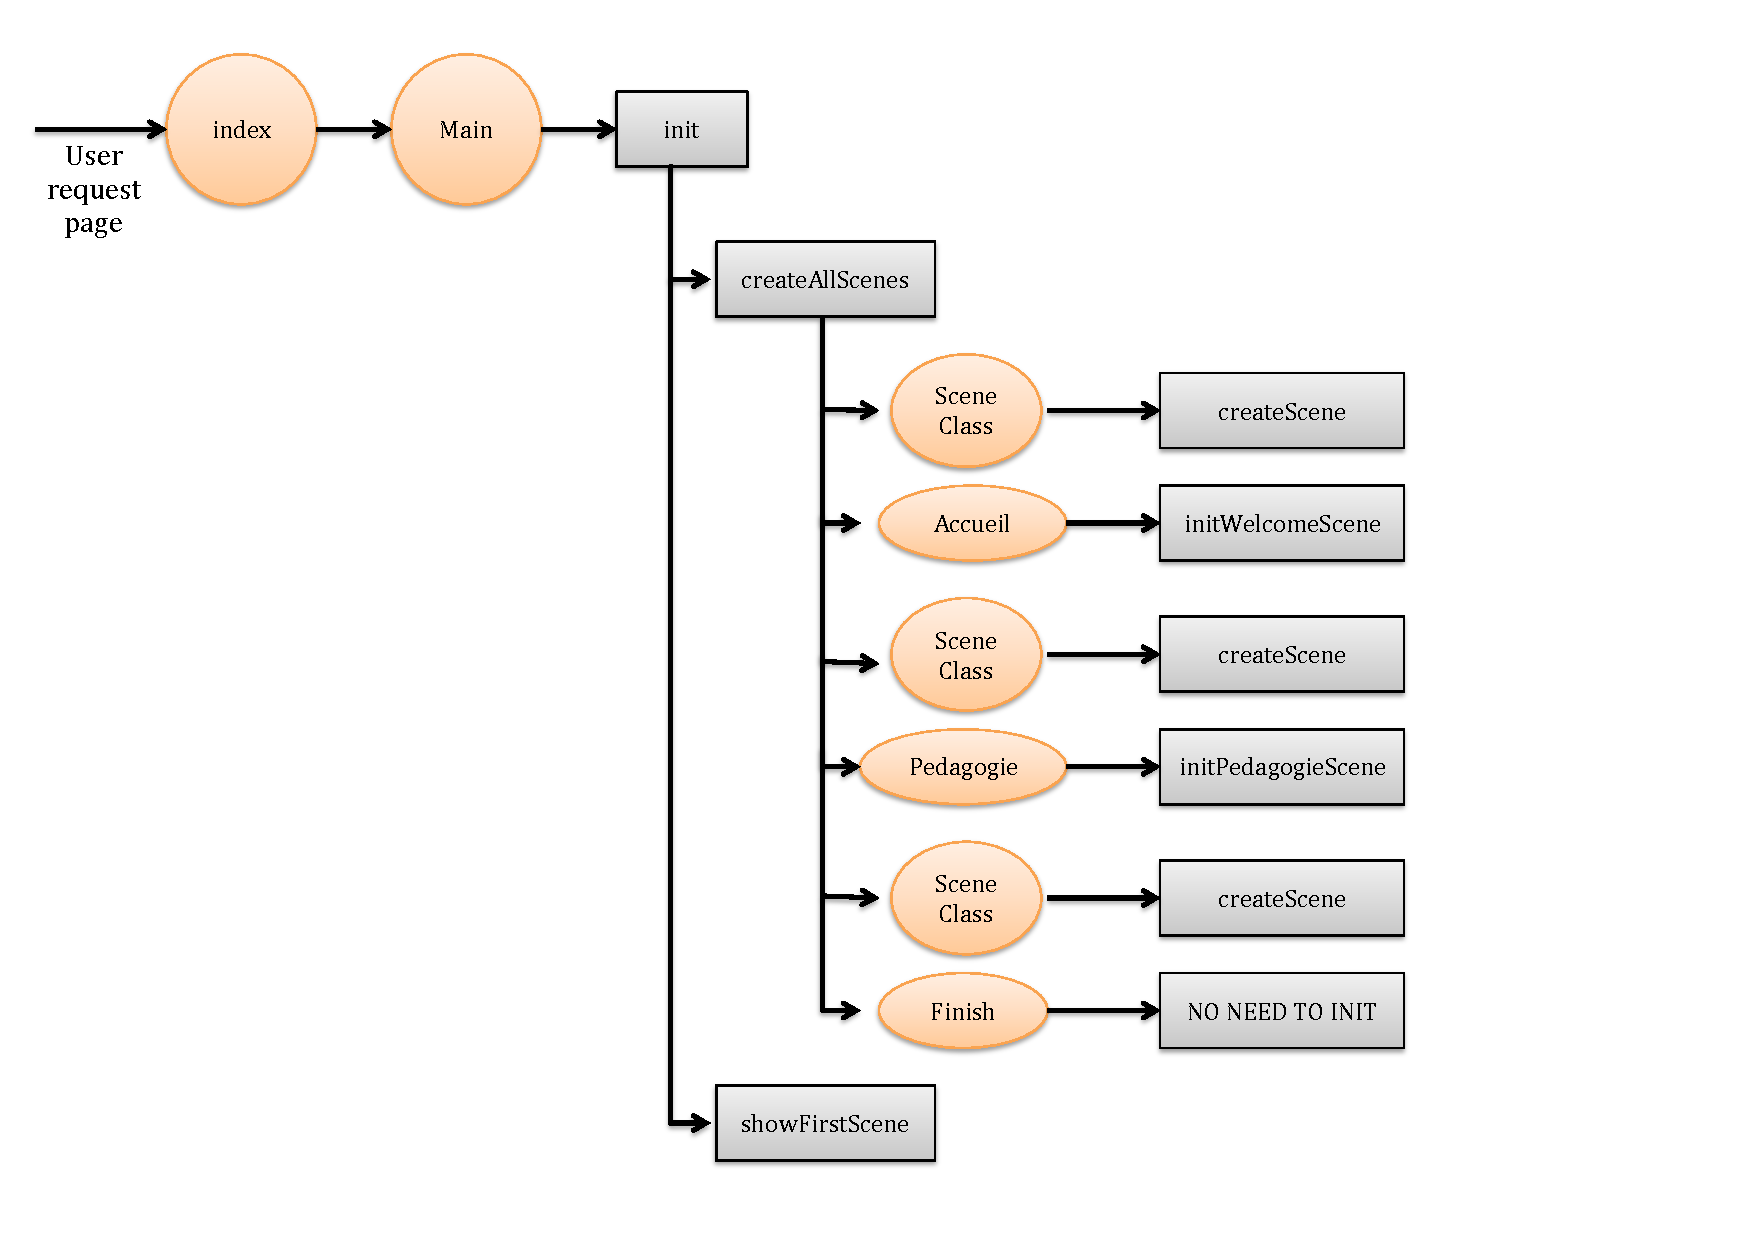
\includegraphics[width=\columnwidth]{images/ScenarioInit.pdf}
\caption{Init web application}
\label{fig:classes}
\end{center}
\end{figure}

\newpage
\subsection{Reaction to a drop in the scene}
\begin{figure}[!h]
\begin{center}
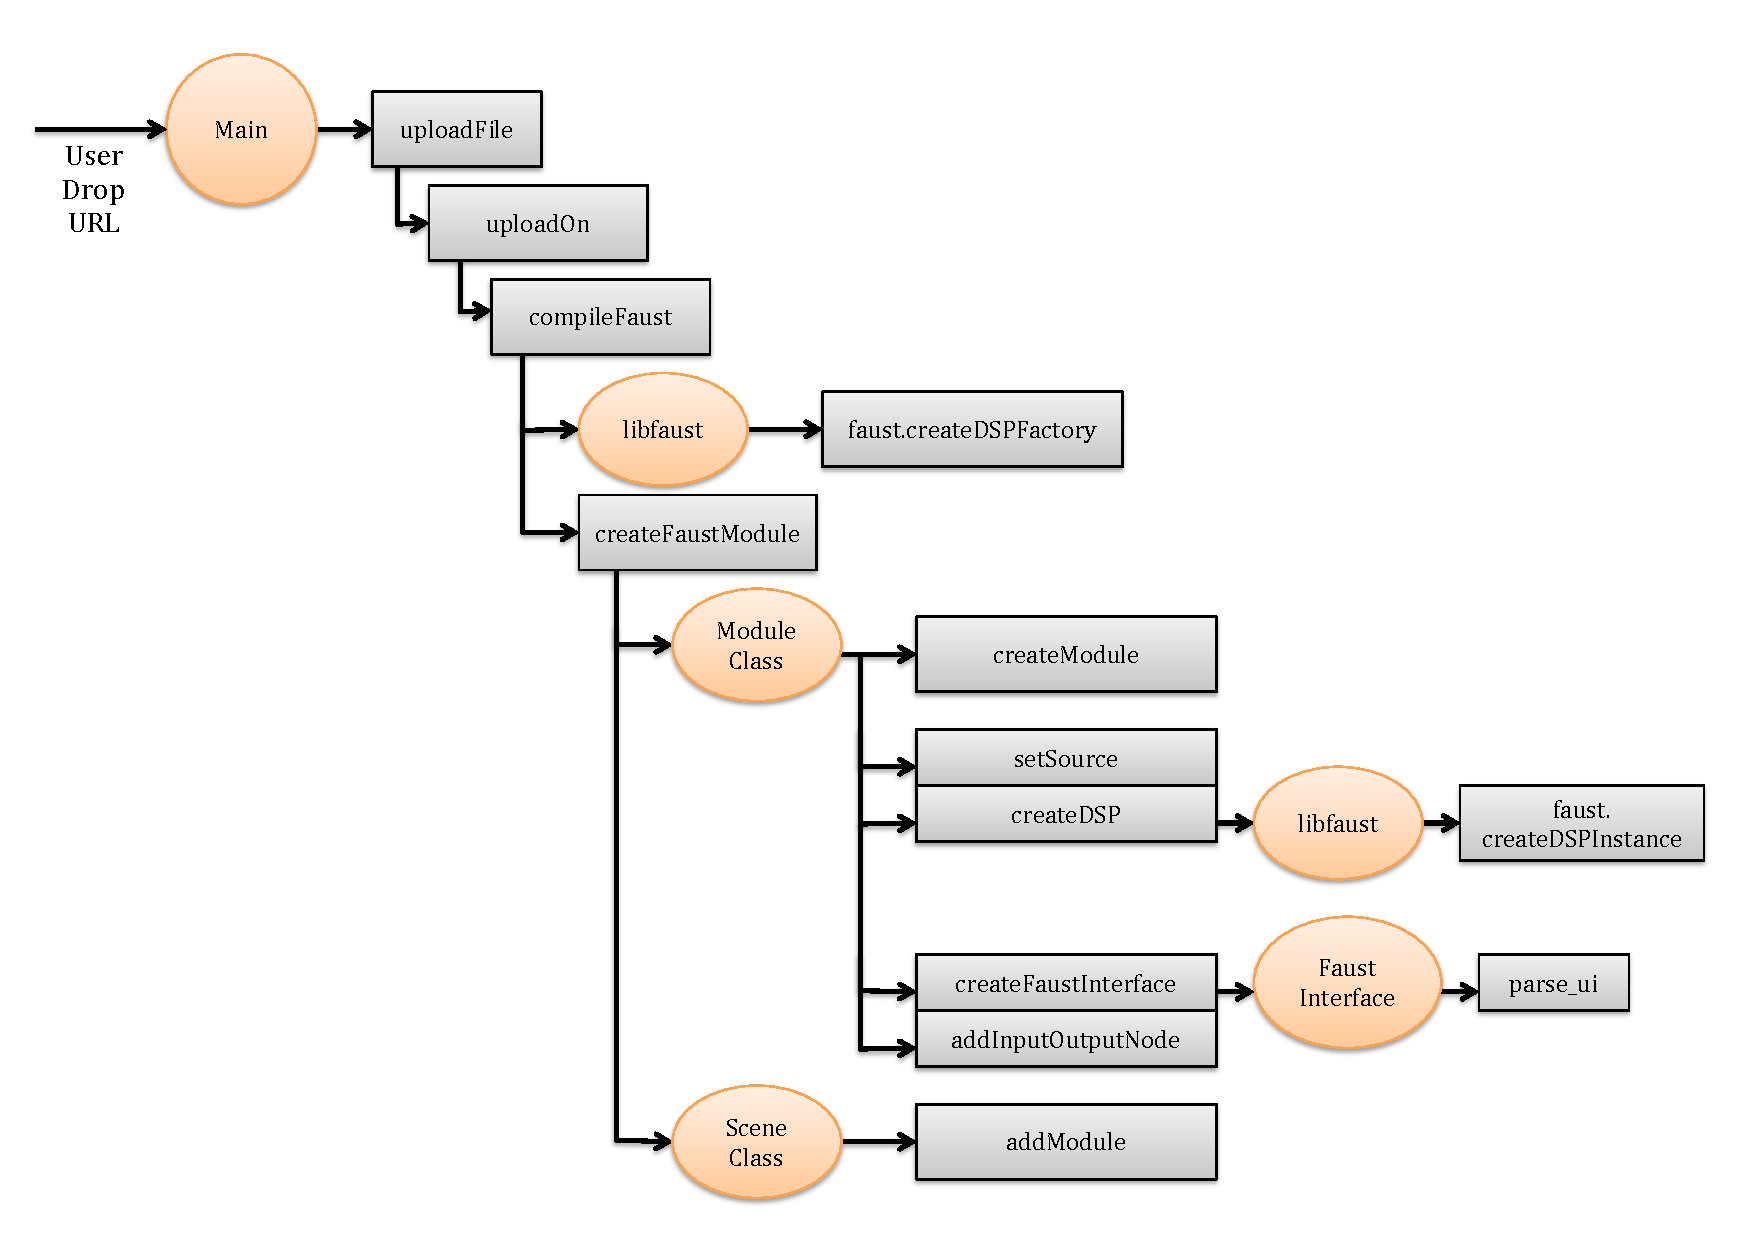
\includegraphics[width=\columnwidth]{images/ScenarioDrop.pdf}
\caption{Drop URL on the scene}
\label{fig:classes}
\end{center}
\end{figure}

\newpage
\subsection{Reaction to a connection drag from the module to the scene output}
\begin{figure}[!h]
\begin{center}
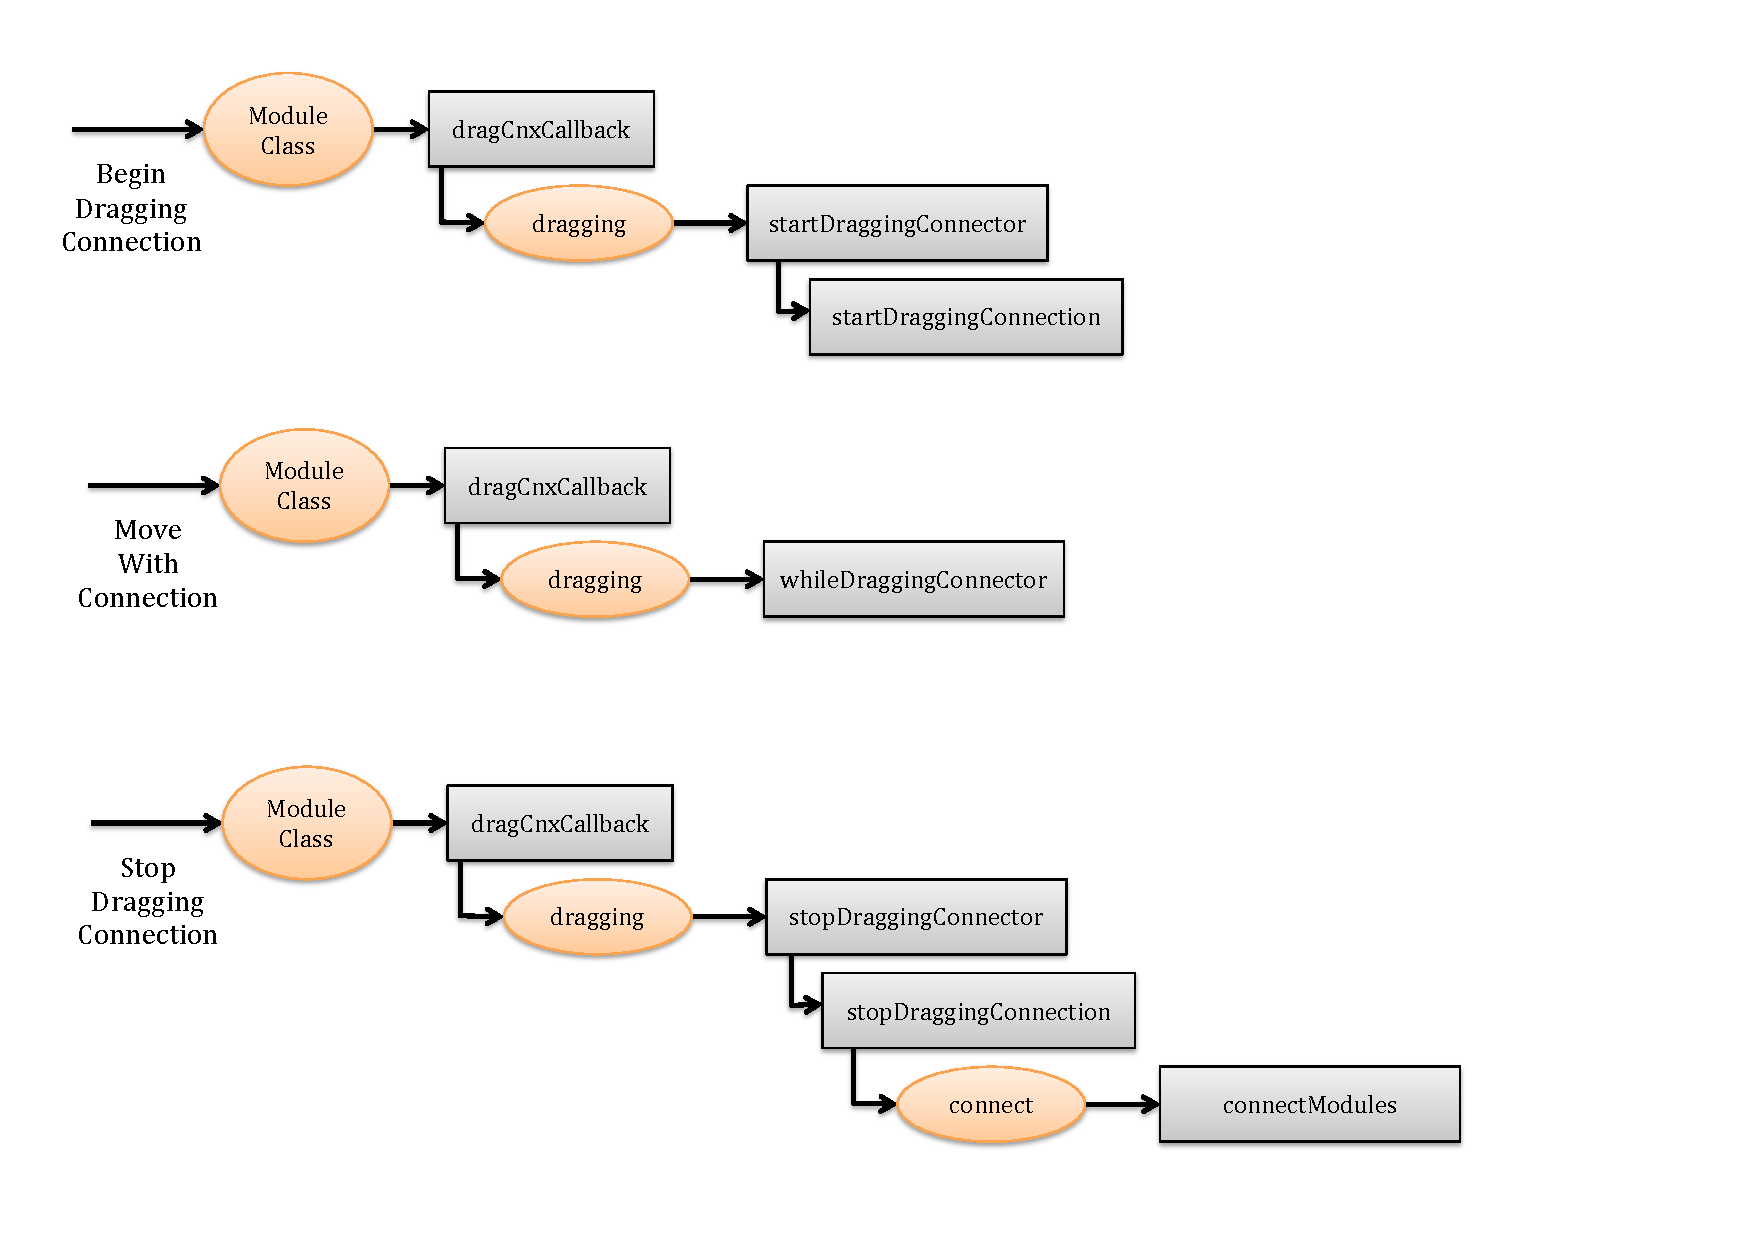
\includegraphics[width=\columnwidth]{images/ScenarioConnect.pdf}
\caption{Connection of a module to the scene output}
\label{fig:classes}
\end{center}
\end{figure}

\newpage
\subsection{Reaction to a source edition}
\begin{figure}[!h]
\begin{center}
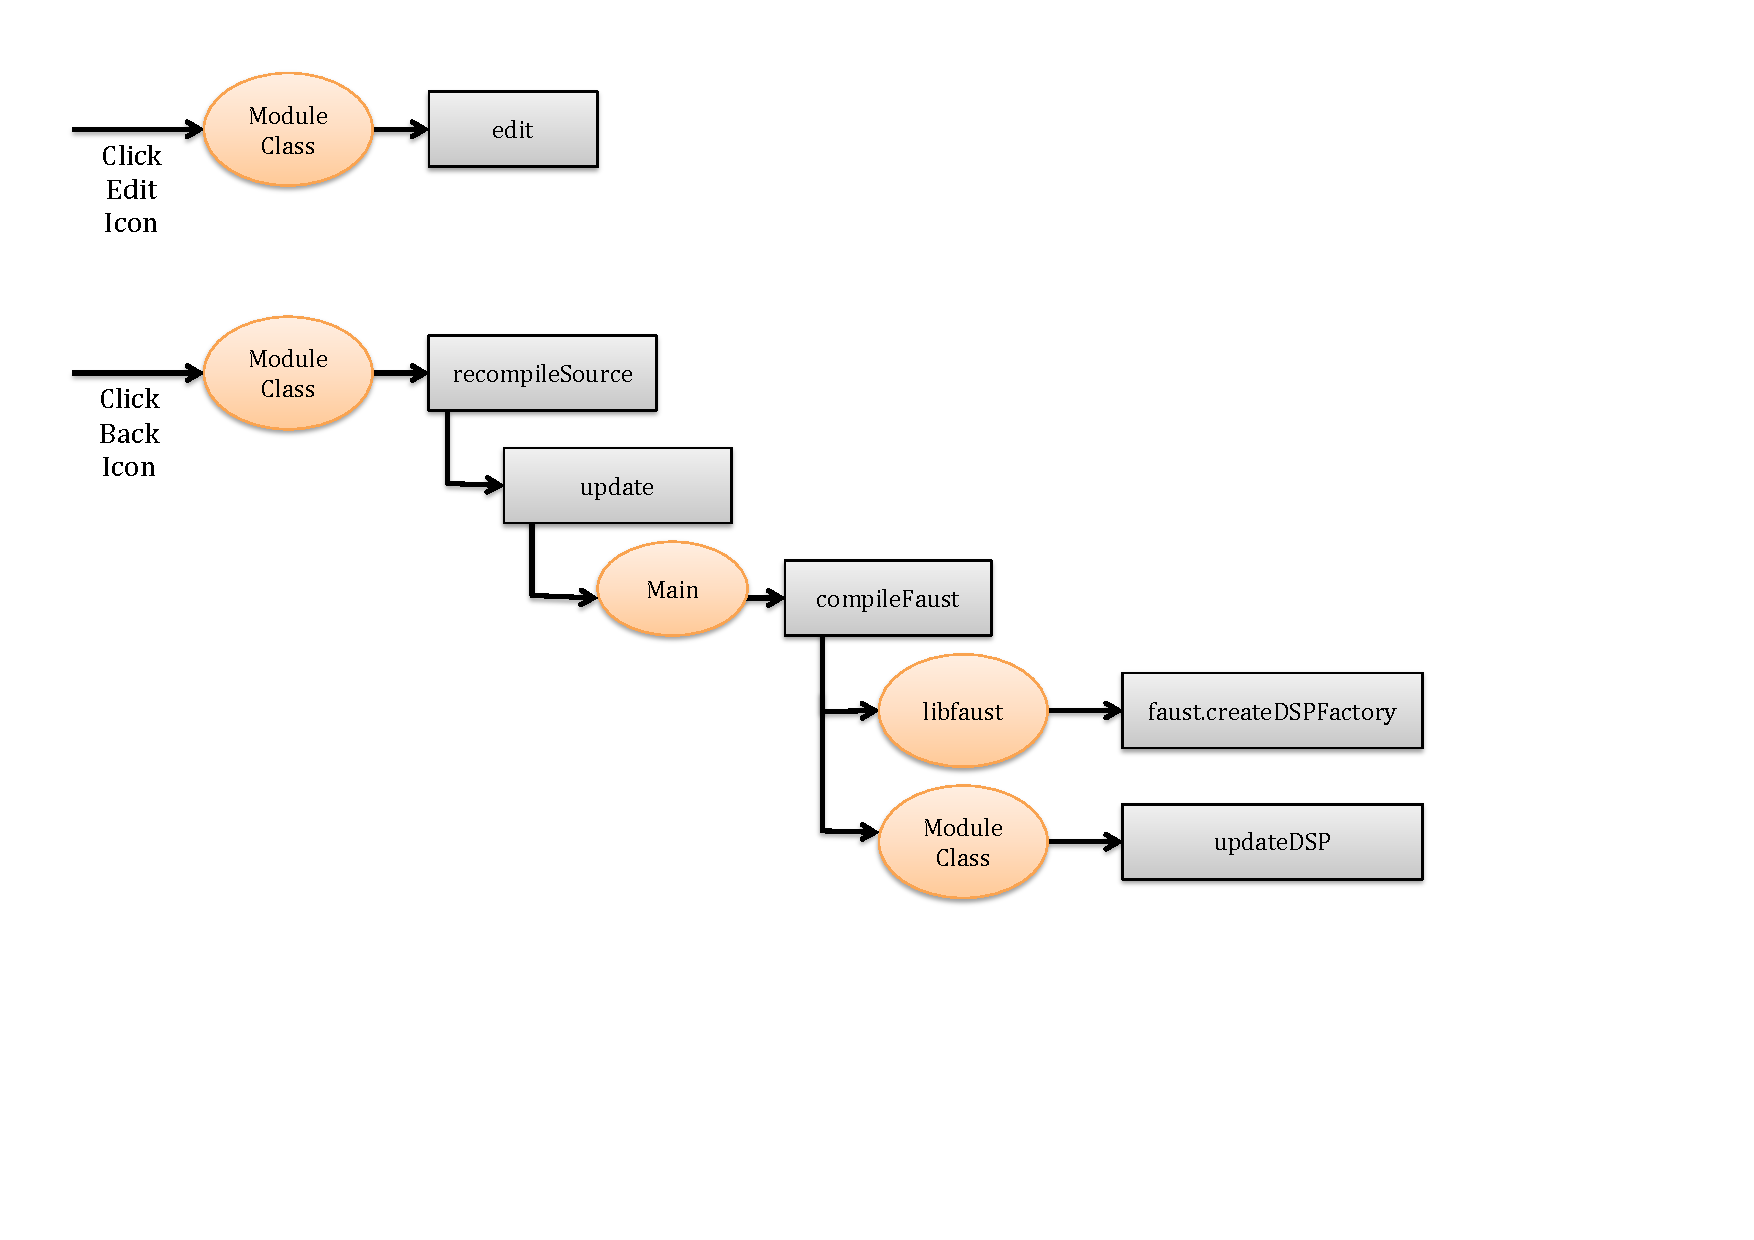
\includegraphics[width=\columnwidth]{images/ScenarioEdit.pdf}
\caption{Edition of a Module Faust Source}
\label{fig:classes}
\end{center}
\end{figure}

\newpage
\section{Appendix}
\subsection{File interactions}
%\begin{landscape}
\begin{figure}[!h]
\begin{center}
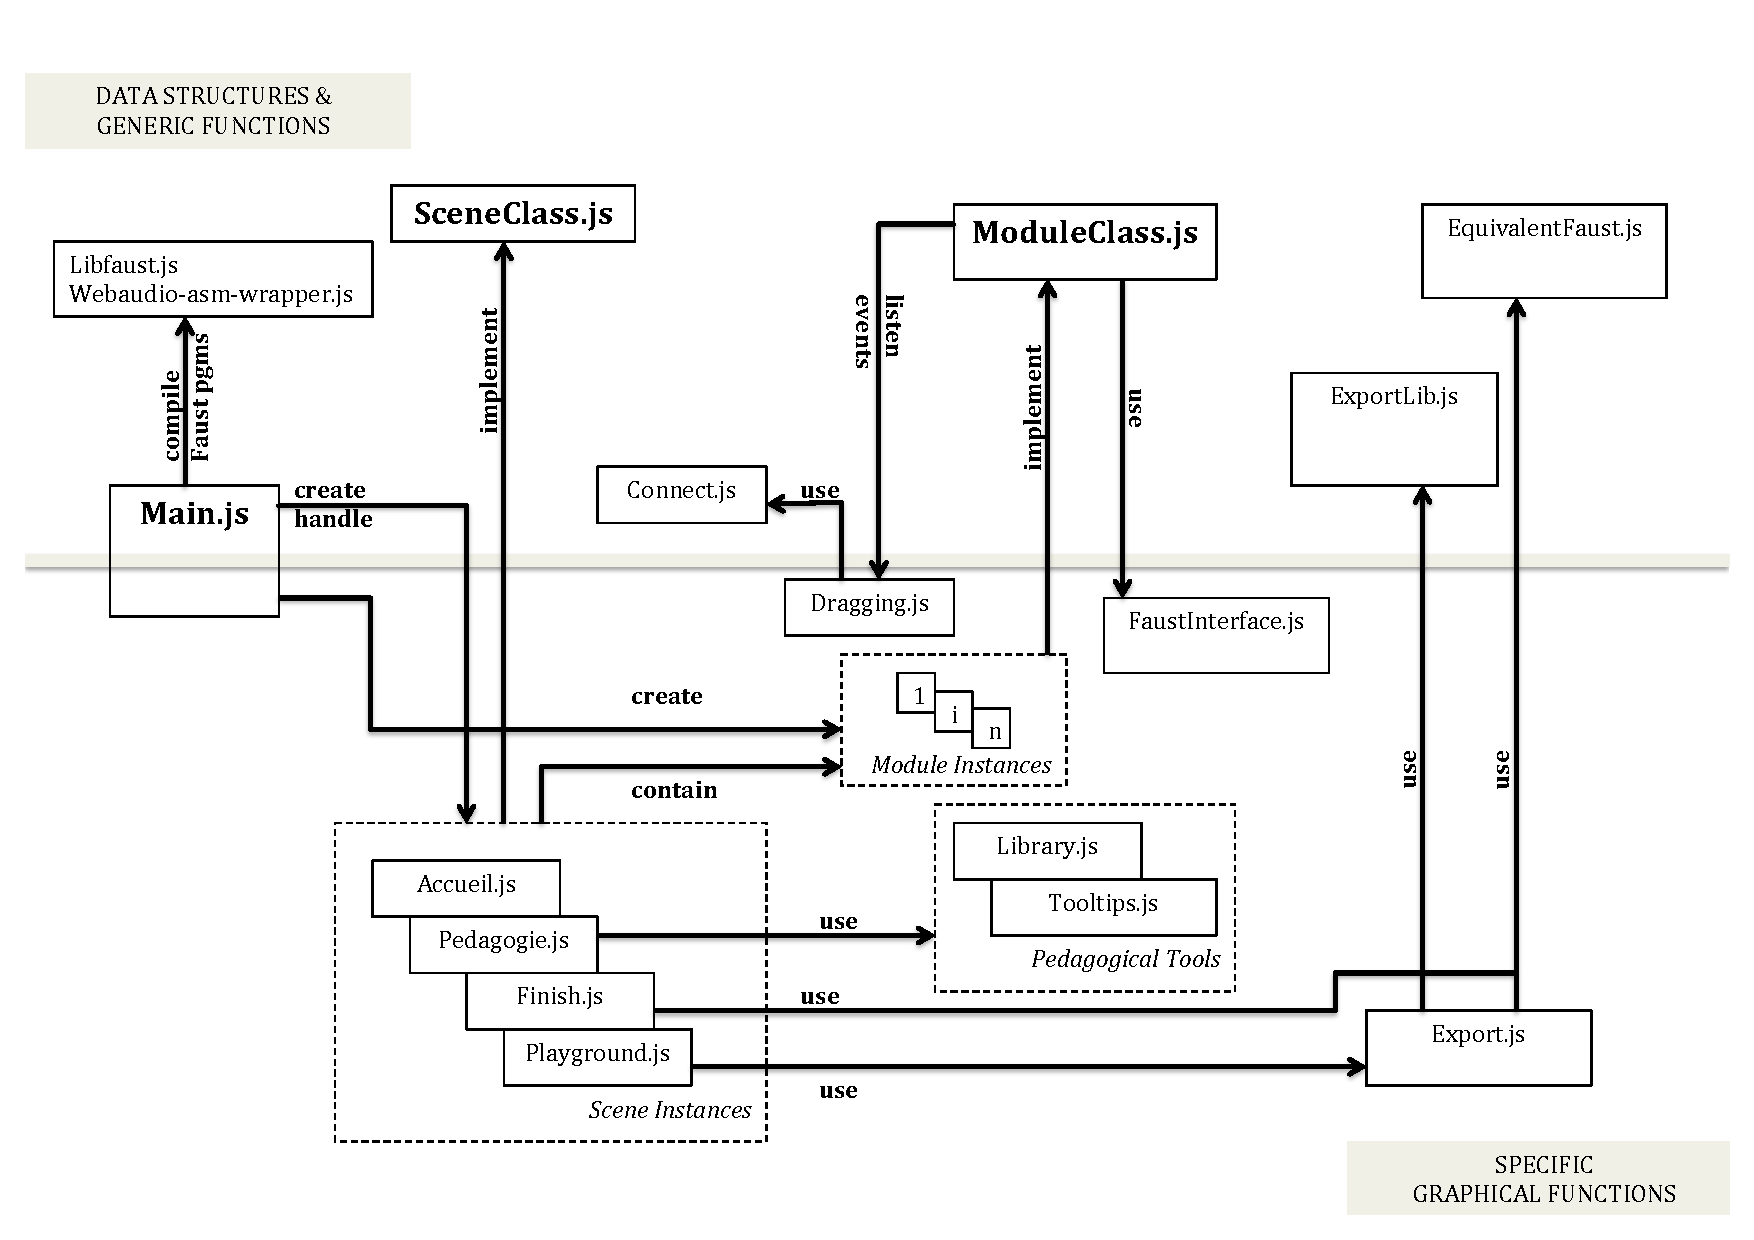
\includegraphics[width=\columnwidth]{images/ClassDiagram.pdf}
\label{fig:classes}
\end{center}
\end{figure}
%\end{landscape}

\newpage
\subsection{JSON Description for the scene}

\begin{figure}[!h]
\begin{center}
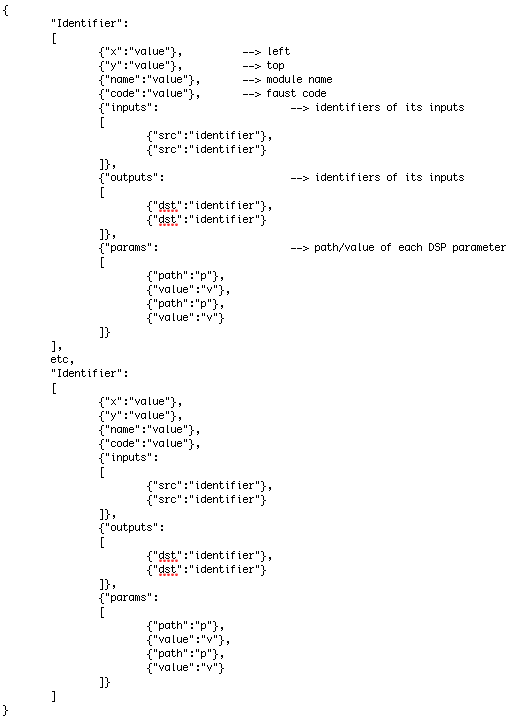
\includegraphics[width=\columnwidth]{images/JSON.png}
\label{fig:JSON}
\end{center}
\end{figure}


\end{document}




